%
% fig-tangentialvektoren.tex
%
% (c) 2025 Prof Dr Andreas Müller
%
\begin{figure}
\centering
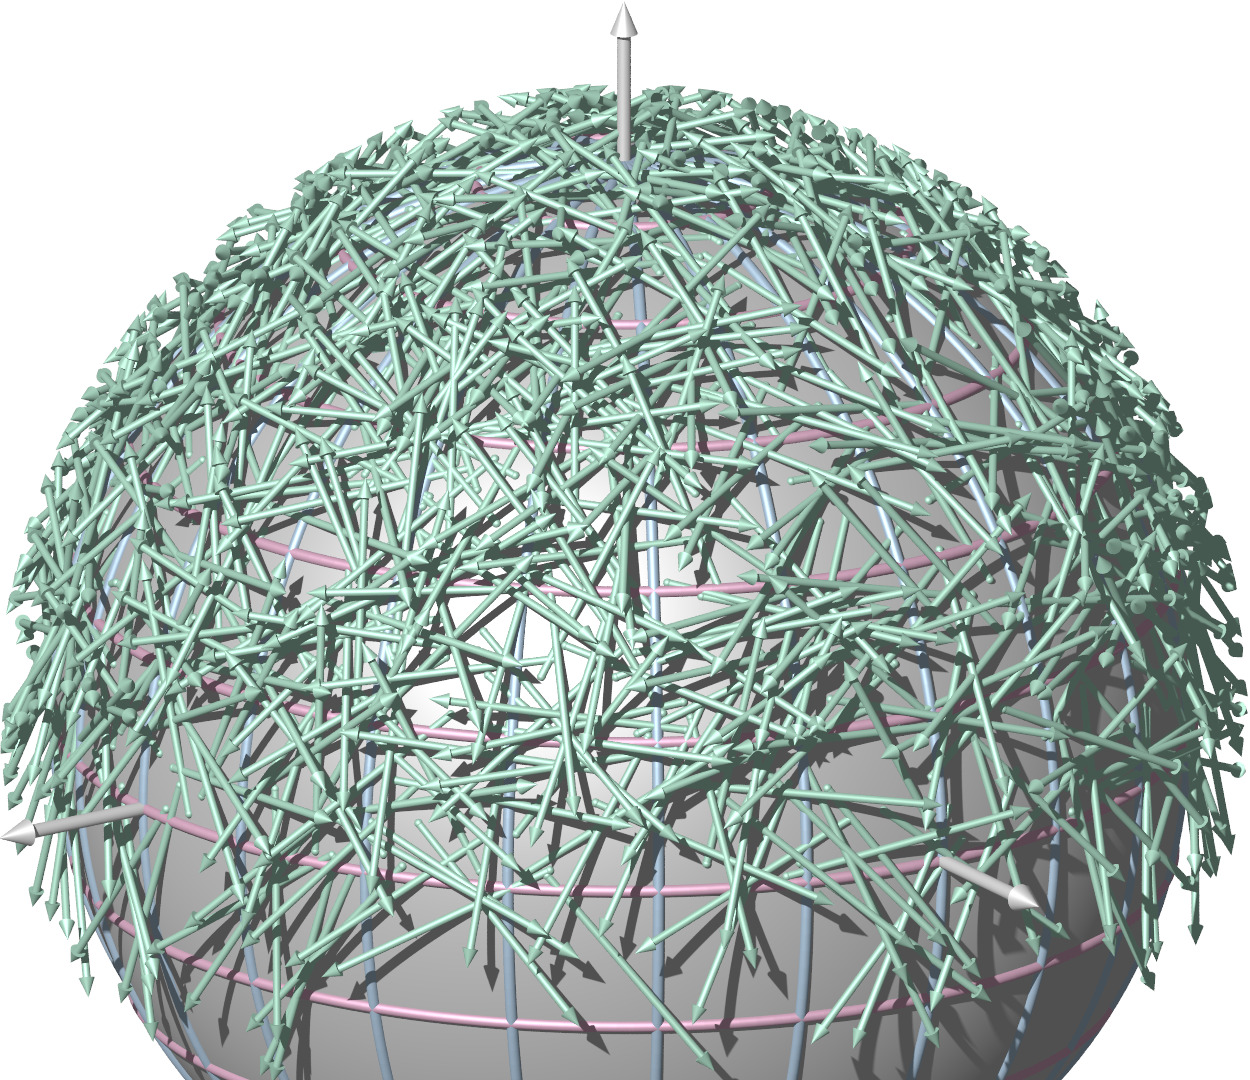
\includegraphics[width=10cm]{chapters/020-koordinaten/images/tangentialvektoren.jpg}
\caption{Darstellung von tausend zufälligen Tangentialvektoren an die
Nordhalbkugel.
Ganz offensichtlich sind die Tangentialvektoren nicht Teil der Kugel.
\label{buch:koordinaten:fig:tangentialvektoren}}
\end{figure}
